% C083: extracted shared teaching figure.
\begin{center}
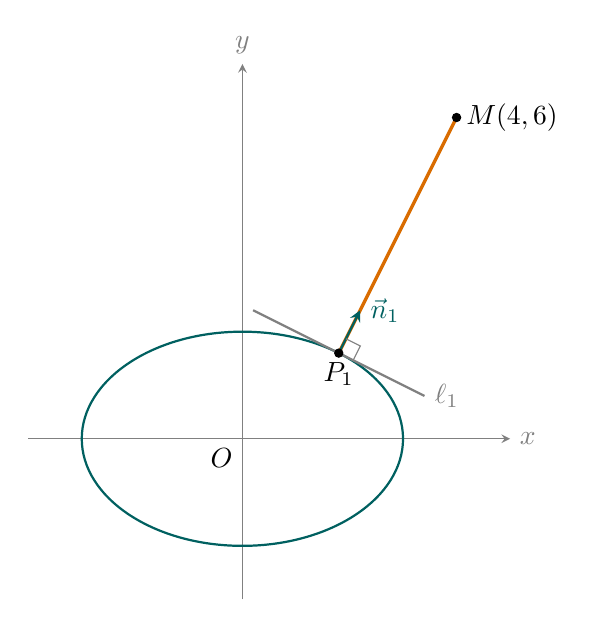
\begin{tikzpicture}[scale=.68,>=stealth]
\draw[->,gray] (-4,0)--(5,0) node[right]{$x$};
\draw[->,gray] (0,-3)--(0,7) node[above]{$y$};
\draw[teal!75!black,thick] (0,0) ellipse (3 and 2);
\coordinate (M) at (4,6); \coordinate (P) at (1.8,1.6);
\draw[orange!85!black,very thick] (P)--(M);
\draw[gray,thick] (.2,2.4)--(3.4,.8) node[right]{$\ell_1$};
\draw[->,teal!75!black,thick] (P)--(2.2,2.4) node[right]{$\vec n_1$};
\draw[gray] (2.068,1.466)--(2.202,1.734)--(1.934,1.868);
\fill (M) circle (2.5pt) node[right]{$M(4,6)$};
\fill (P) circle (2.5pt) node[below]{$P_1$};
\node[below left] at (0,0) {$O$};
\end{tikzpicture}
\end{center}
